\myslide{Outline - Übersicht}
{
  \begin{itemgroup}{}
    \item Von Ausdrücken und Typen kann der Ableitungsbaum betrachtet werden
          (z.B. $\TypeArrowType{\TypeIntegerType}{\TypeArrowType{\TypeIntegerType}{\TypeIntegerType}}$)
    \item Schwierige Ausdrucke können so besser verstanden werden
    \item Name der Ausdücke und Typen wird dargestellt (z.B. Let)
    \item Menge der Ausdrücke und Typen wird dargestellt (z.B. op)
    \item Der Index der Kinder wird eingeblendet (z.B. $e_1$)
    \item Bindungen von Identifiern (z.B. $\ExprLet{\ExprIdentifierBinding{x}}{}{\ExprConstant{2}}
          {\ExprInfixOperation{\ExprBinaryOperator{+}}{\ExprIdentifierBound{x}}{\ExprConstant{1}}}$)
    \item Die Outline muss bei neu implementierten Ausdrücken nicht angepasst
          werden, sondern übernimmt diese automatisch
  \end{itemgroup}
}

\myslide{Outline - Einstellungen}
{
  \begin{itemgroup}{}
    \item \textbf{Hervorheben}: Selektierte Knoten werden in höheren Knoten farblich 
                                hervorgehoben
    \item \textbf{Gebundene}: Gebundene Identifier werden markiert
    \item \textbf{Freie}: Frei vorkommende Identifier werden markiert
    \item \textbf{Ersetzen}: Selektierte Knoten werden in höheren Knoten durch
                             \glqq\textbf{...}\grqq\ ersetzt, dadurch wird die Ansicht
                             kompakter
    \item \textbf{Source Code}: Der zu dem selektierten Knoten passende Source Code
                                wird im Editor hervorgehoben
    \item \textbf{Auto Update}: Die Outline wird bei Änderungen automatisch aktualisiert
                                (z.B. Änderungen im Source Code Editor)
  \end{itemgroup}
}

\myslide{Outline - Beispiel}
{
  \begin{center}
    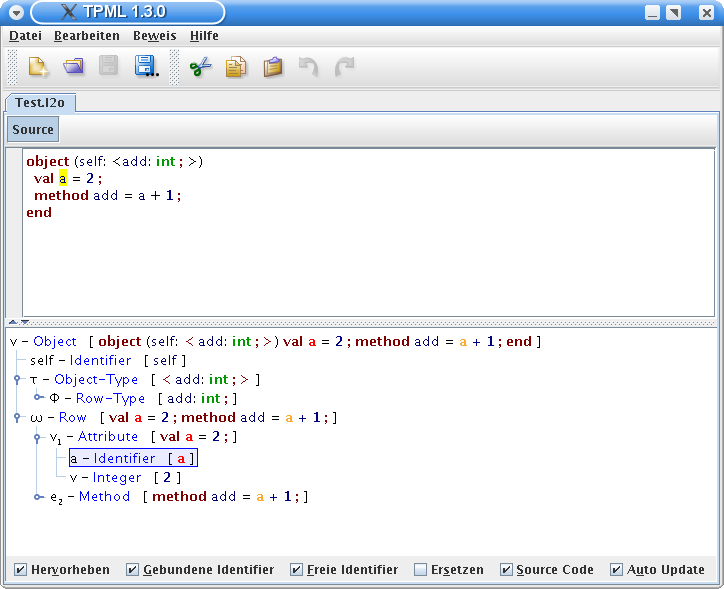
\includegraphics[height=14cm]{images/outline.png}
  \end{center}
}